% ==========================================================
% Document setup
% ==========================================================
\documentclass{article}
\usepackage[margin=1.5cm, top=1cm]{geometry}

% ==========================================================
% Imported packages
% ==========================================================
\usepackage{graphicx}   % Figures
\usepackage{subcaption} % Subfigures
\usepackage{booktabs}   % Nice tables
\usepackage{amsmath}    % Equations
\usepackage{amssymb}    % Math symbols

% ==========================================================
% Notation commands
% ==========================================================
\newcommand{\PDMATLAB}{\texttt{PDMATLAB2D}}
\newcommand{\R}{\mathbb{R}}
\newcommand{\C}{\mathbb{C}}
\newcommand{\expect}{\mathbb{E}}
\newcommand{\inputspace}{\mathcal{U}}
\newcommand{\outputspace}{\mathcal{V}}
\newcommand{\inputdimension}{d}
\newcommand{\outputdimension}{d}
\newcommand{\inputdomain}{{\Omega_\inputspace}}
\newcommand{\outputdomain}{{\Omega_\outputspace}}
\newcommand{\inputvecdim}{{c_\inputspace}}
\newcommand{\inputcodomain}{\R^\inputvecdim}
\newcommand{\outputvecdim}{{c_\outputspace}}
\newcommand{\outputcodomain}{\R^\outputvecdim}
\newcommand{\inputdiscdimension}{m}
\newcommand{\outputdiscdimension}{n}
\newcommand{\inputdiscretization}{D_{\inputspace}}
\newcommand{\outputdiscretization}{D_{\outputspace}}
\newcommand{\inputdiscspace}{\mathscr{D}(\inputspace)}
\newcommand{\outputdiscspace}{\mathscr{D}(\outputspace)}
\newcommand{\opdiscspace}{\mathscr{D}(\inputspace, \outputspace)}
\newcommand{\effectivediscspace}{\mathscr{ED}(\inputspace,\outputspace)}
\renewcommand{\vec}[1]{\mathbf{#1}}
\newcommand{\bs}{\boldsymbol}
\newcommand{\trueop}{G^\dagger}
\newcommand{\modelparam}{\theta}
\newcommand{\model}[1]{G_{#1}}  % #1 = parameters
\newcommand{\deeponet}{\model{\modelparam}^{\text{DeepONet}}}
\newcommand{\ear}{\model{\modelparam}^\text{EAR}}
\newcommand{\fno}{\model{\modelparam}^\text{FNO}}
\newcommand{\gnot}{\model{\modelparam}^\text{GNOT}}
\newcommand{\ourmodel}{G_\textnormal{ours}}
\newcommand{\numericalmodelnaked}[1]{\widetilde{G}_{#1}}  % #1 = parameters
\newcommand{\numericalmodel}[5][]{\numericalmodelnaked{#2}#1(#3, #4; #5#1)}  % #1 = size hint for delimiters, #2 = parameters, #3 = input discretization, #4 = output discretization, #5 = input
\newcommand{\dataelem}[2]{{#1}^{(#2)}} % #1 = data, #2 = index
\newcommand{\mat}[1]{\left[\begin{matrix}#1\end{matrix}\right]}
\newcommand{\risk}{\mathcal{R}}
\newcommand{\emprisk}{\widehat{\mathcal{R}}}
\newcommand{\inputlatentdim}{p}
\newcommand{\outputlatentdim}{q}
\newcommand{\encoder}{E}
\newcommand{\approximator}{A}
\newcommand{\reconstructor}{R}
\newcommand{\encoderparams}{\theta_E}
\newcommand{\approxparams}{\theta_A}
\newcommand{\reconstructparams}{\theta_R}
\newcommand{\encodernet}{\Phi^E}
\newcommand{\approxnet}{\Phi^A}
\newcommand{\reconstructnet}{\Phi^R}
\newcommand{\variance}{\mathrm{Var}}
\newcommand{\proj}{\mathrm{proj}}
\newcommand{\tr}{\mathrm{tr}}
\newcommand{\dee}{\;\mathrm{d}}
\newcommand{\fourier}{\mathscr{F}}
\newcommand{\dfourier}{\mathscr{F}_\text{p}}
\newcommand{\mybox}[1]{%
	\noindent\fbox{%
		\parbox{\textwidth}{#1}
	}
}

% ==========================================================
% Title
% ==========================================================
\title{SCGSR Final Report Additional Materials}
\author{Jacob Hauck}
\date{August 30, 2026}

% ==========================================================
% Document
% ==========================================================
\begin{document}
	
	\maketitle
	
	% ==========================================================
	% Figure 1
	% ==========================================================
	\begin{figure}[htb!]
		\centering
		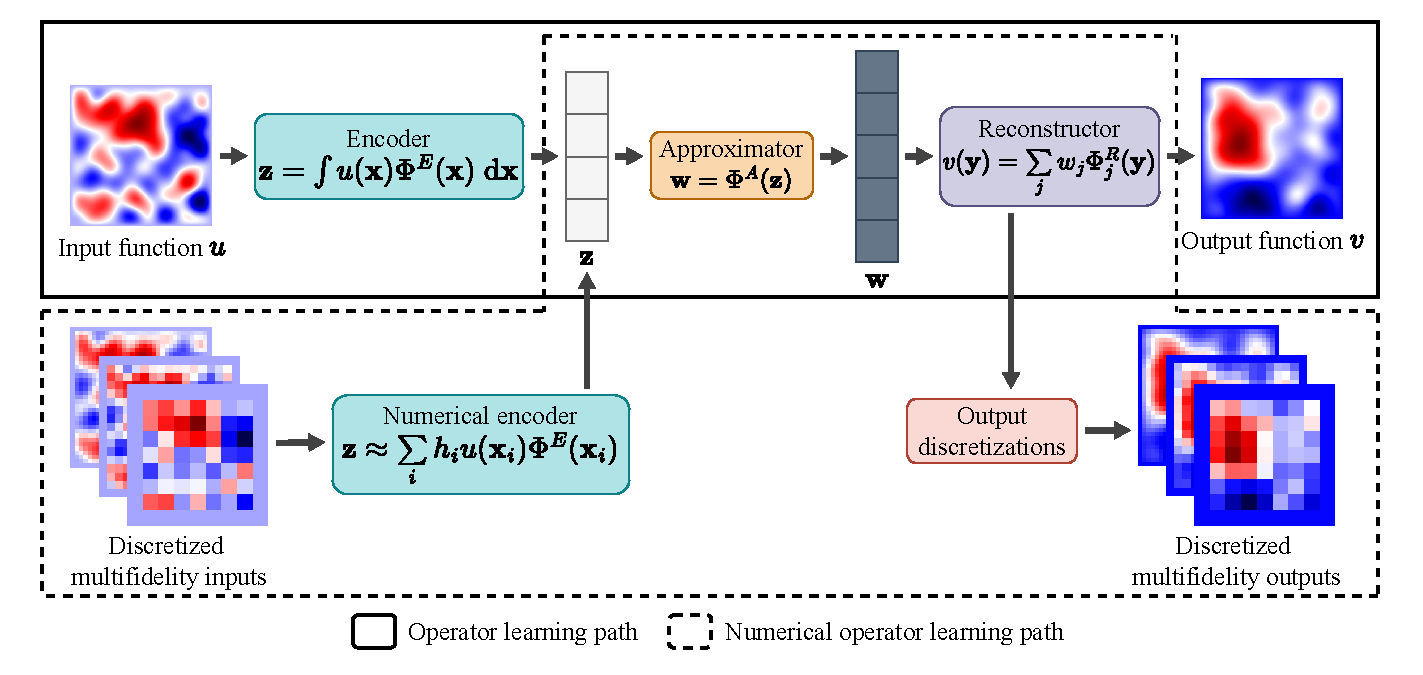
\includegraphics[width=\linewidth]{figures/operator_learning_diagram.pdf}
		\caption{The architecture of our operator learning method, and how operator learning enables discretization independence through numerical operator learning. Note the three-module structure: (linear) encoder projects the input function onto a finite-dimensional space parameterized by neural network basis functions ($\Phi^E$), approximator approximates the operator in the latent space, and (linear) reconstructor builds the output function by taking a linear combination of neural network basis functions (using a different neural network $\Phi^R$) using the latent output variables from the approximator as weights. Vector-valued extension is described in \eqref{eq:extension}.}
	\end{figure}
	
	% ==========================================================
	% Equation 1
	% ==========================================================
	
	\begin{equation}
		\label{eq:extension}
		\begin{gathered}
			\begin{cases}
				\encoder(\encoderparams; u) = \big(\langle u, \encodernet_1\rangle,  \ldots,  \langle u, 	\encodernet_{\inputlatentdim}\rangle\big) \in \R^{\inputlatentdim}, &\qquad u\in \inputspace = L^2(\inputdomain; \R^{\inputvecdim}),\\[0.3em]
				\approximator(\approxparams; \vec{z}) = \approxnet(\vec{z}) \in \R^{\outputlatentdim}, 	&\qquad\vec{z}\in \R^{\inputlatentdim},\\[0.3em]
				\reconstructor(\reconstructparams; \vec{w}) = \sum\limits_{j=1}^{\outputlatentdim}w_j 	\reconstructnet_j \, \in \outputspace = L^2(\outputdomain; \R^\outputvecdim), &\qquad\vec{w}\in\R^{\outputlatentdim},
			\end{cases} \\[0.5em]
			\text{where} \\[0.5em]
			\encodernet(\vec{x}) = \mat{\varphi_1^E(\vec{x}) \\ \varphi_2^E(\vec{x}) \\ \vdots \\ 	\varphi_\inputlatentdim^E(\vec{x})}, \quad \vec{x} \in \inputdomain, \qquad \reconstructnet(\vec{y}) = \mat{\varphi_1^R(\vec{y}) \\ \varphi_2^R(\vec{y}) \\ \vdots \\ \varphi_\outputlatentdim^R(\vec{y})}, \quad \vec{y} \in \outputdomain,\\[0.5em]
			\varphi_i^E : \inputdomain \to \R^\inputvecdim, \qquad \varphi_i^R : \outputdomain \to \R^\outputvecdim.
		\end{gathered}
	\end{equation}
	
	
	% ==========================================================
	% Figure 2
	% ==========================================================
	\begin{figure}[htb!]
		\centering
		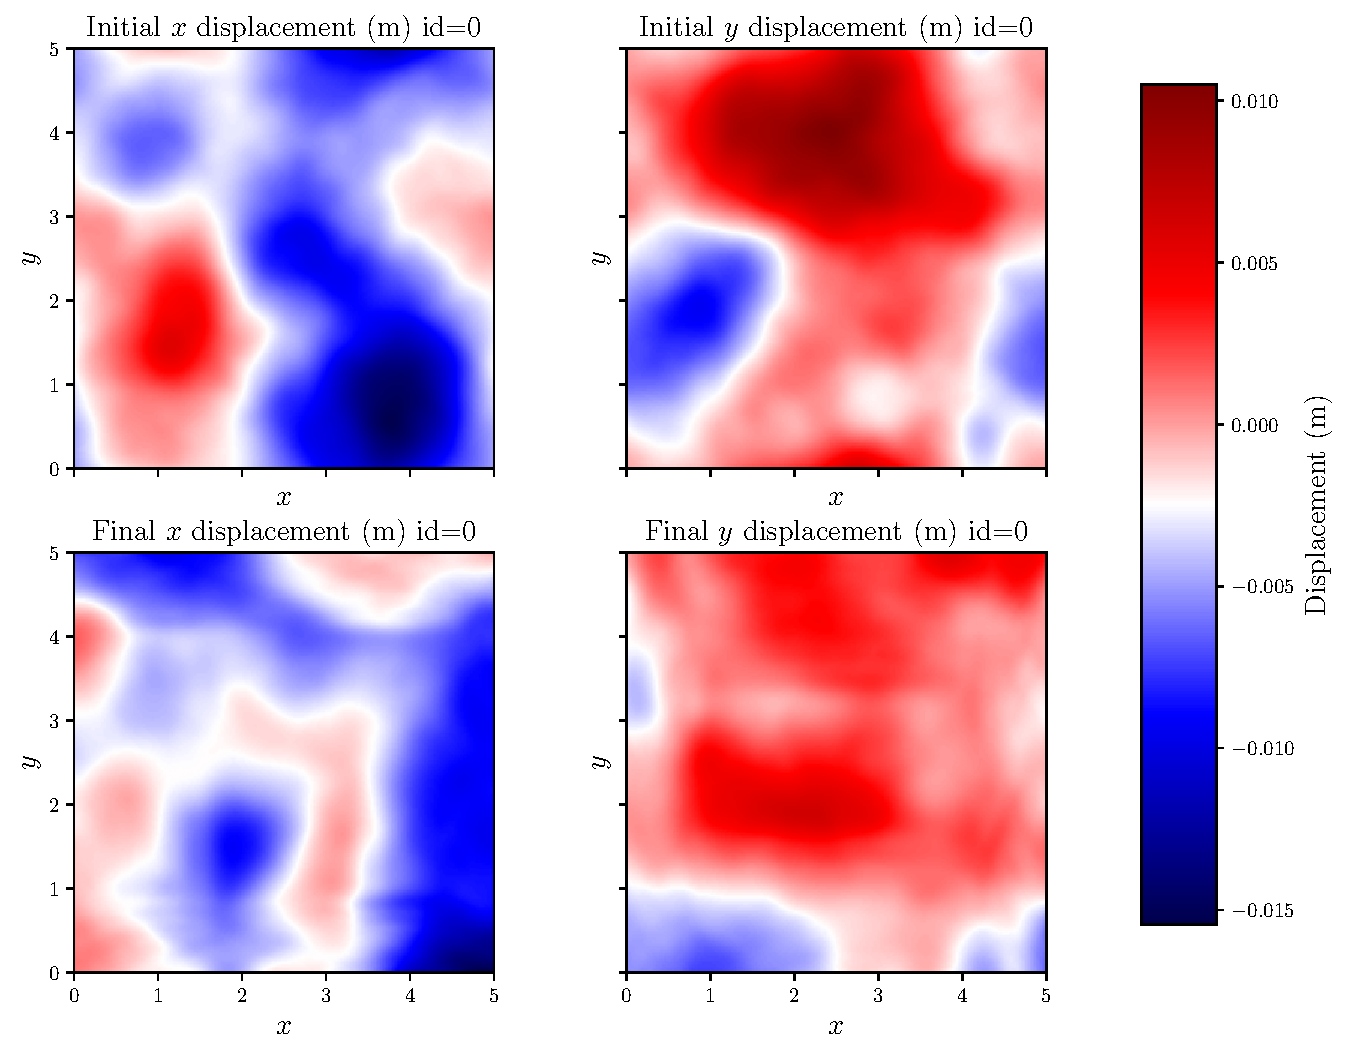
\includegraphics[width=0.8\linewidth]{figures/example_wave_data.pdf}
		\caption{Example input--output pair from one of the wave propagation benchmark datasets, prepared using \texttt{PDMATLAB2D}. The input function is the top row, which shows the initial $x$ and $y$ displacement fields. The output function is the bottom row, which shows the final $x$ and $y$ displacement fields after a time $T = 1.8$ seconds has elapsed in the simulation. The ``id=0'' refers to this sample's ID in the dataset.}
	\end{figure}
	
	
	% ==========================================================
	% Table 1
	% ==========================================================
	\begin{table}[htb!]
		\centering
		\begin{tabular}{@{}lrr@{}}
			\toprule
			Approximator & Error on training data & Error on testing data \\ 
			\midrule
			Base (3 layers, 128 neurons/layer, ReLU) & 15.2 & 18.1 \\ 
			Wide (3 layers, 384 neurons/layer, ReLU) & 12.4 & 20.7 \\
			Deep (8 layers, 128 neurons/layer, SELU) & 11.9 & 16.9 \\
			\bottomrule
		\end{tabular}
		\caption{Error (measured in \% relative $L^2$) for different approximator network settings. Using a wide approximator leads to overfitting (note gap between train and test error in the second row), but using a deep approximator with self-normalizing activation leads to a slight performance boost (compare error in first and third rows).}
	\end{table}
	
	% ==========================================================
	% Figure 3
	% ==========================================================
	\begin{figure}[htb!]
		\centering
		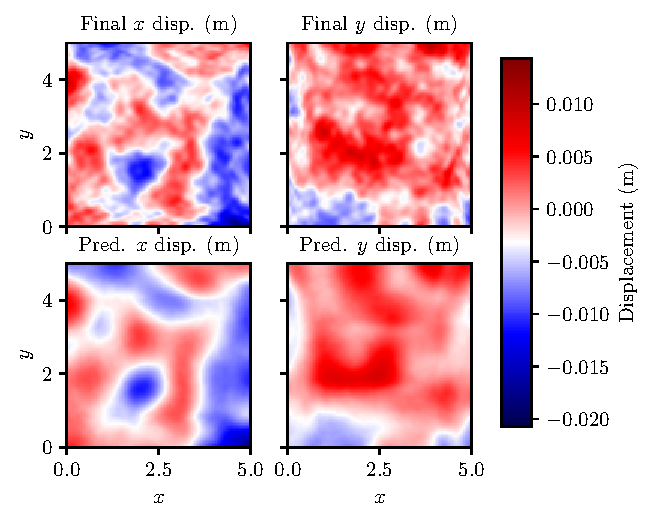
\includegraphics[width=0.5\linewidth]{figures/test17_tg.ol.h5_pred_0.pdf}
		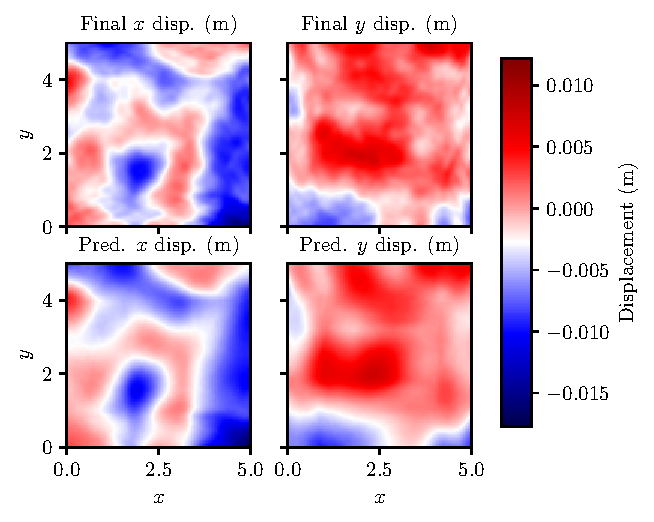
\includegraphics[width=0.5\linewidth]{figures/test19_tg.ol.h5_pred_0.pdf}
		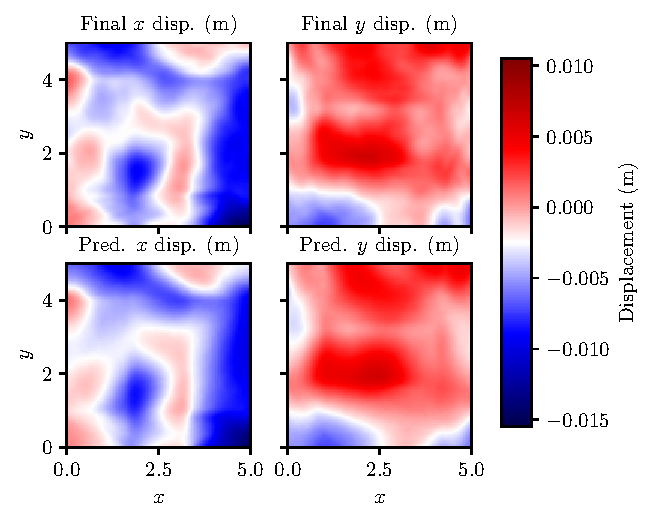
\includegraphics[width=0.5\linewidth]{figures/test21_tg.ol.h5_pred_0.pdf}
		\caption{Example final displacement fields (top rows, $x$ and $y$ components alternating) and corresponding model predictions (bottom rows) for different input Gaussian process covariance eigenvalue decay rates. Decay rate increases from top to bottom. Note the corresponding decrease in strong high-frequency components from top to bottom. Also note how the model prediction only capture low-frequency (smooth) components, making its predictions more accurate when the covariance eigenvalues decay quickly.}
	\end{figure}
	
	
	% ==========================================================
	% Table 2
	% ==========================================================
	\begin{table}[htb!]
		\centering
		\begin{tabular}{@{}lrr@{}}
			\toprule
			$\gamma$ & Error on training data & Error on testing data \\ 
			\midrule
			2.5 & 14.3 & 18.6 \\
			3.1 & 7.6 & 10.7 \\
			4.0 & 4.6 & 7.1 \\
			5.0 & 4.0 & 5.7 \\
			\bottomrule
		\end{tabular}
		\caption{Error (measured in \% relative $L^2$) for different input distribution complexities, as measured by the $\gamma$ decay rate of the covariance eigenvalues; smaller $\gamma$ means more complex. We observe that the more complex data is more difficult for operator learning models to fit, as measured both on the training and testing data.}
	\end{table}
	
	% ==========================================================
	% Figure 4
	% ==========================================================
	\begin{figure}[htb!]
		\centering
		\begin{subfigure}[t]{0.49\linewidth}
			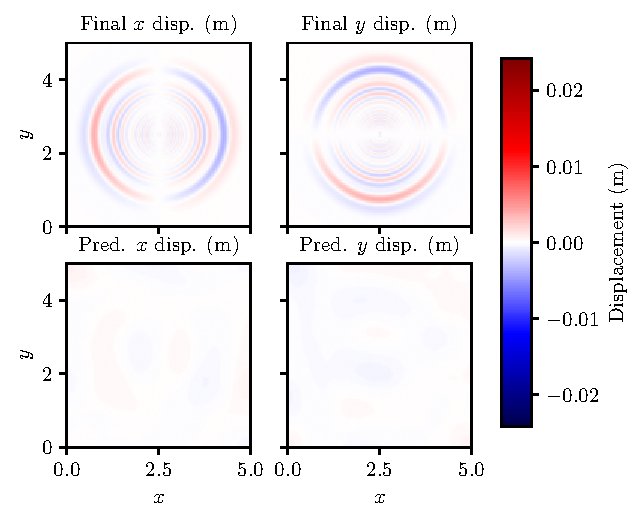
\includegraphics[width=\linewidth]{figures/BumpProp1.ol.h5_pred_0.pdf}
			\subcaption{Initial displacement size = $0.03$}
		\end{subfigure}
		~
		\begin{subfigure}[t]{0.49\linewidth}
			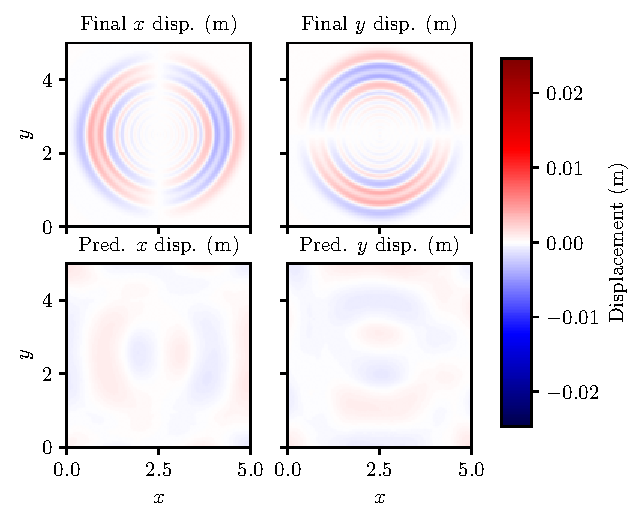
\includegraphics[width=\linewidth]{figures/BumpProp5.ol.h5_pred_0.pdf}
			\subcaption{Initial displacement size = $0.05$}
		\end{subfigure}
		~
		\begin{subfigure}[t]{0.49\linewidth}
			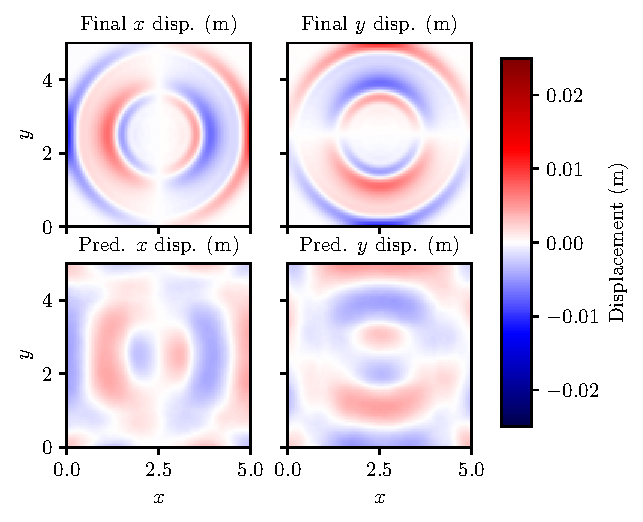
\includegraphics[width=\linewidth]{figures/BumpProp4.ol.h5_pred_0.pdf}
			\subcaption{Initial displacement size = $0.10$}
		\end{subfigure}
		~
		\begin{subfigure}[t]{0.49\linewidth}
			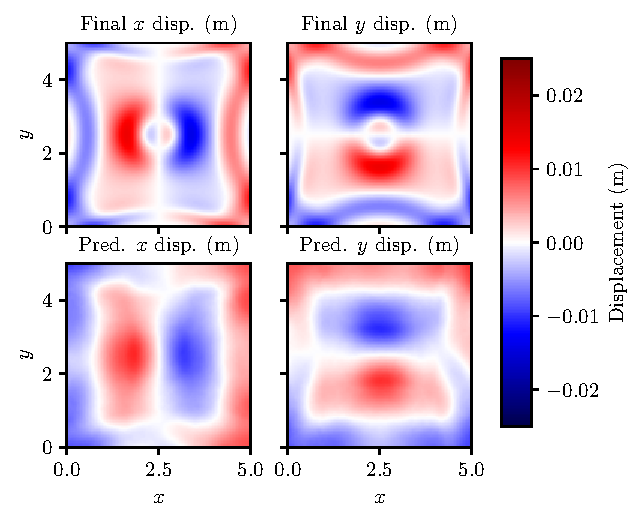
\includegraphics[width=\linewidth]{figures/BumpProp3.ol.h5_pred_0.pdf}
			\subcaption{Initial displacement size = $0.20$}
		\end{subfigure}
		~
		\begin{subfigure}[t]{0.5\linewidth}
			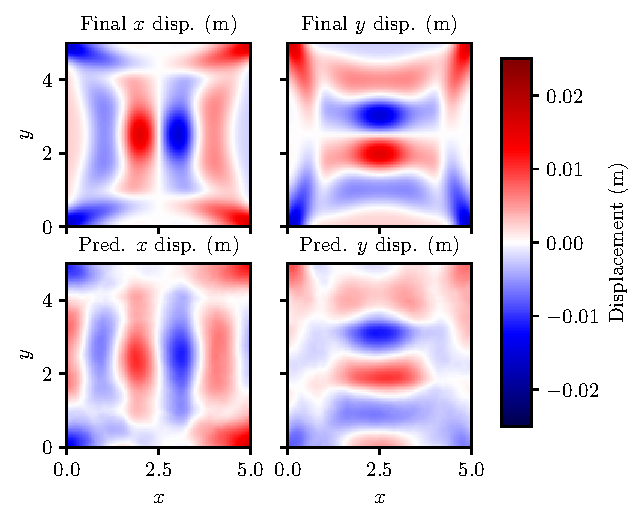
\includegraphics[width=\linewidth]{figures/BumpProp2.ol.h5_pred_0.pdf}
			\subcaption{Initial displacement size = $0.30$}
		\end{subfigure}
		\caption{Model predictions for out-of-distribution initial displacements. The top rows in each block show simulation final displacement field $x$ and $y$ components, and the bottom rows show the corresponding model predictions. Input initial displacement fields are Gaussian bumps of varying sizes, specified in the captions of each subfigure. The model makes more accurate predictions for larger bumps (which have less high-frequency information and result in less dispersive effects).}
	\end{figure}
	
	% ==========================================================
	% Table 3
	% ==========================================================
	\begin{table}[htb!]
		\centering
		\begin{tabular}{@{}rrr@{}}
			\toprule
			$T$ & Error on training data & Error on testing data \\
			\midrule
			1.8 & 15.4 & 18.2 \\
			1.4 & 16.5 & 21.0 \\
			1.0 & 16.0 & 19.3 \\
			0.6 & 14.1 & 17.1 \\
			0.2 & 14.4 & 19.2 \\
			\bottomrule
		\end{tabular}
		\caption{Independence of model error (measured in \% relative $L^2$) on simulation duration $T$. When $T = 0.2$, the operator is nearly the identity, suggesting that the reconstructor module in our model is insufficient. As illustrated in Figure \ref{fig:model_size}, the error of our model can be reduced by increasing the number of basis functions in the encoder and reconstructor.}
	\end{table}
	
	% ==========================================================
	% Figure 5
	% ==========================================================
	\begin{figure}[htb!]
		\centering
		\begin{subfigure}[t]{0.49\linewidth}
			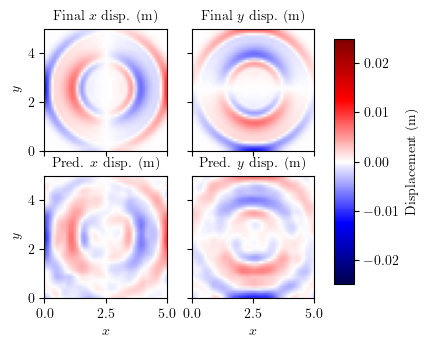
\includegraphics[width=\textwidth]{figures/BumpProp4_50_256.png}
			\subcaption{256 basis functions}
		\end{subfigure}
		~
		\begin{subfigure}[t]{0.49\linewidth}
			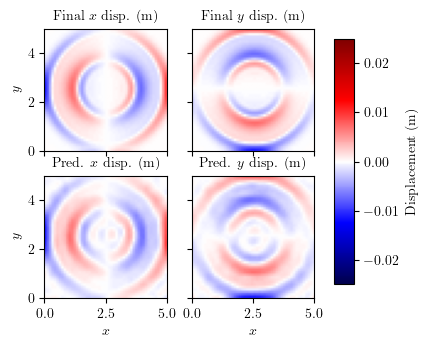
\includegraphics[width=\textwidth]{figures/BumpProp4_50_512.png}
			\subcaption{512 basis functions}
		\end{subfigure}
		~
		\begin{subfigure}[t]{0.49\linewidth}
			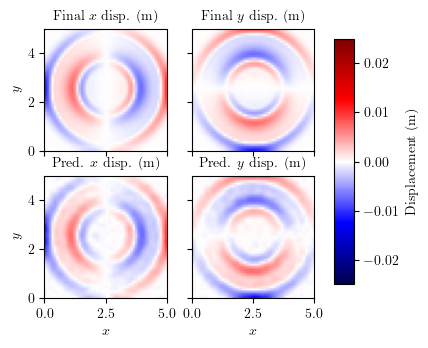
\includegraphics[width=\textwidth]{figures/BumpProp4_1024.png}
			\subcaption{1024 basis functions}
		\end{subfigure}
		\caption{Model predictions for out-of-distribution for initial displacements for different model sizes compared to true final states (top rows), as measured by the number of basis functions in the encoder/reconstructor modules ($p$ and $q$ in \eqref{eq:extension}). We need to increase the number of basis functions substantially in order to achieve good accuracy, which is a symptom of the challenges of hyperbolic problems (such as elasticity) for operator learning. Note that even fewer basis functions (128) were used in Figure 4, which explains why the accuracy there is even lower than in any of the above cases.}
		\label{fig:model_size}
	\end{figure}
	
	% ==========================================================
	% Figure 6
	% ==========================================================
	\begin{figure}[htb!]
	\centering
	\begin{subfigure}[t]{0.49\linewidth}
		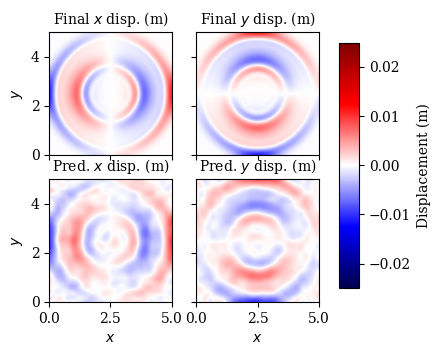
\includegraphics[width=\textwidth]{figures/waveIso_tg.ol.h5_pred_0.png}
		\subcaption{Isotropic symmetry}
	\end{subfigure}
	~
	\begin{subfigure}[t]{0.49\linewidth}
		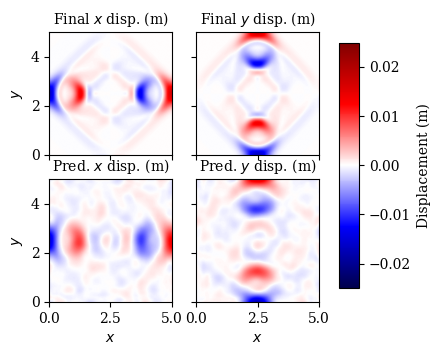
\includegraphics[width=\textwidth]{figures/waveSquare_tg.ol.h5_pred_0.png}
		\subcaption{Square symmetry}
	\end{subfigure}
	~
	\begin{subfigure}[t]{0.49\linewidth}
		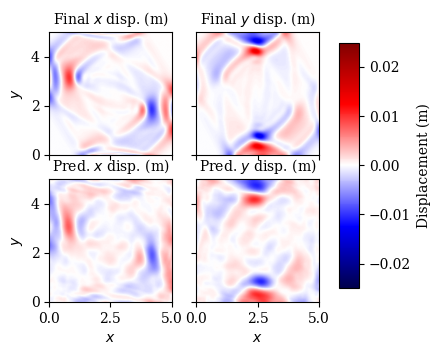
\includegraphics[width=\textwidth]{figures/waveOblique_tg.ol.h5_pred_0.png}
		\subcaption{Oblique symmetry}
	\end{subfigure}
	\caption{Final conditions under different material symmetry models resulting from the same initial condition, along with operator learning predictions from models trained on datasets with corresponding symmetry. Top rows: true final states. Bottom rows: operator learning predictions. We observe similar accuracy across all symmetry types.}
	\end{figure}
	
	
	% ==========================================================
	% Figure 7
	% ==========================================================
	\begin{figure}[htb!]
		\centering
		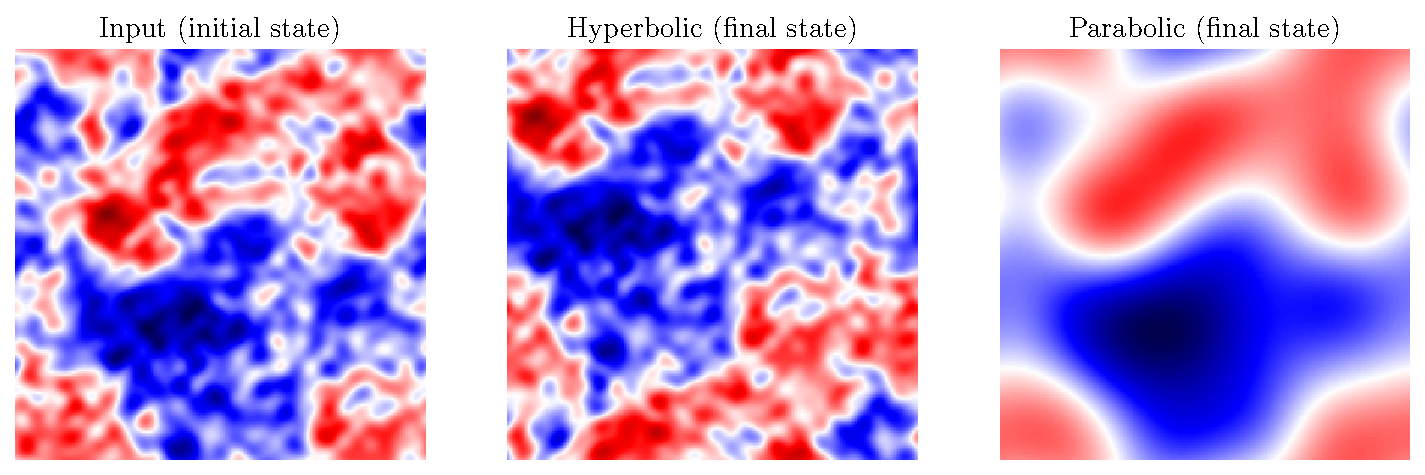
\includegraphics[width=\textwidth]{figures/hyperbolic_vs_parabolic.pdf}
		\caption{Comparison of propagation operators for hyperbolic and parabolic systems. The final state in the hyperbolic problem retains complex (high-frequency) features in the initial state whereas the final state in the parabolic problem is significantly simpler, with all the fine details smoothed out.}
	\end{figure}
	
	
	% ==========================================================
	% Figure 8
	% ==========================================================
	\begin{figure}[htb!]
		\centering
		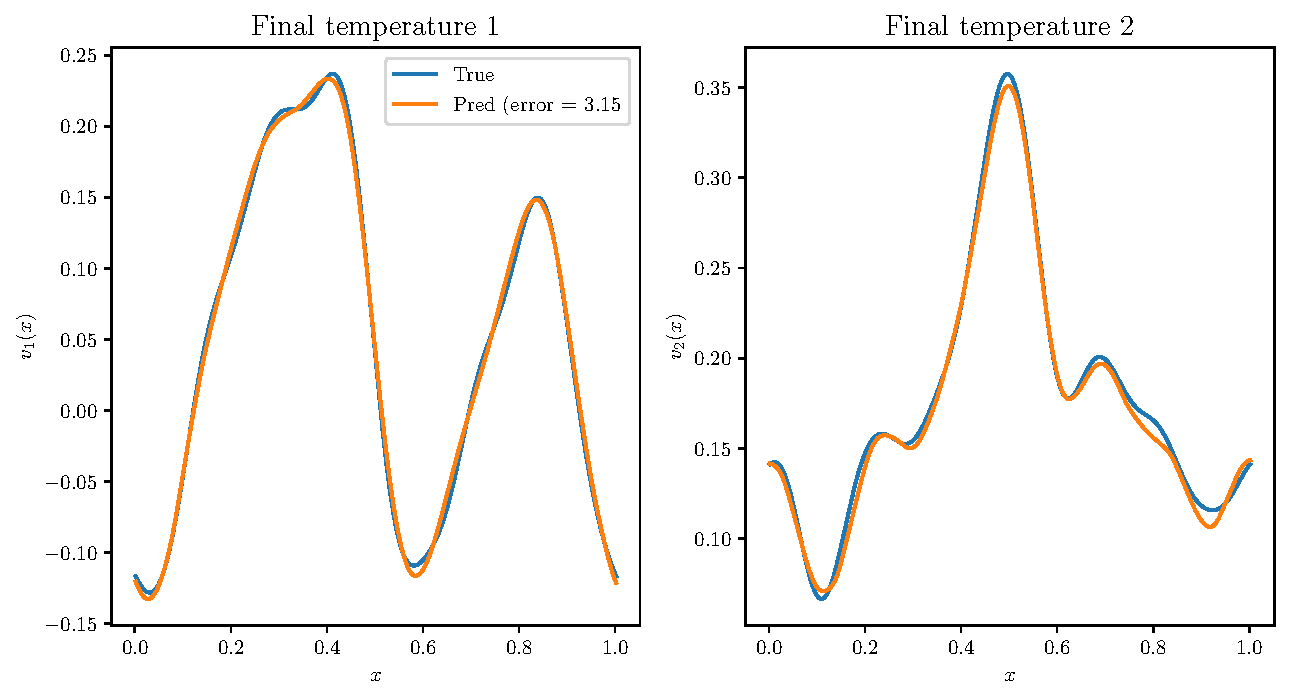
\includegraphics[width=\linewidth]{figures/heat_T=1.2.pdf}
		\caption{Example final state in the 1D heat equation for two samples (labeled temperature 1 and temperature 2 above, as the state in the heat equation is a temperature field rather than a displacement field). We can see that the final states are smoother than in the wave case in Figure \ref{fig:wave_1d}, and the operator learning model makes quite accurate predictions (3.15\% relative $L^2$ error).}
		\label{fig:heat_1d}
	\end{figure}
	
	% ==========================================================
	% Figure 9
	% ==========================================================
	\begin{figure}[htb!]
		\centering
		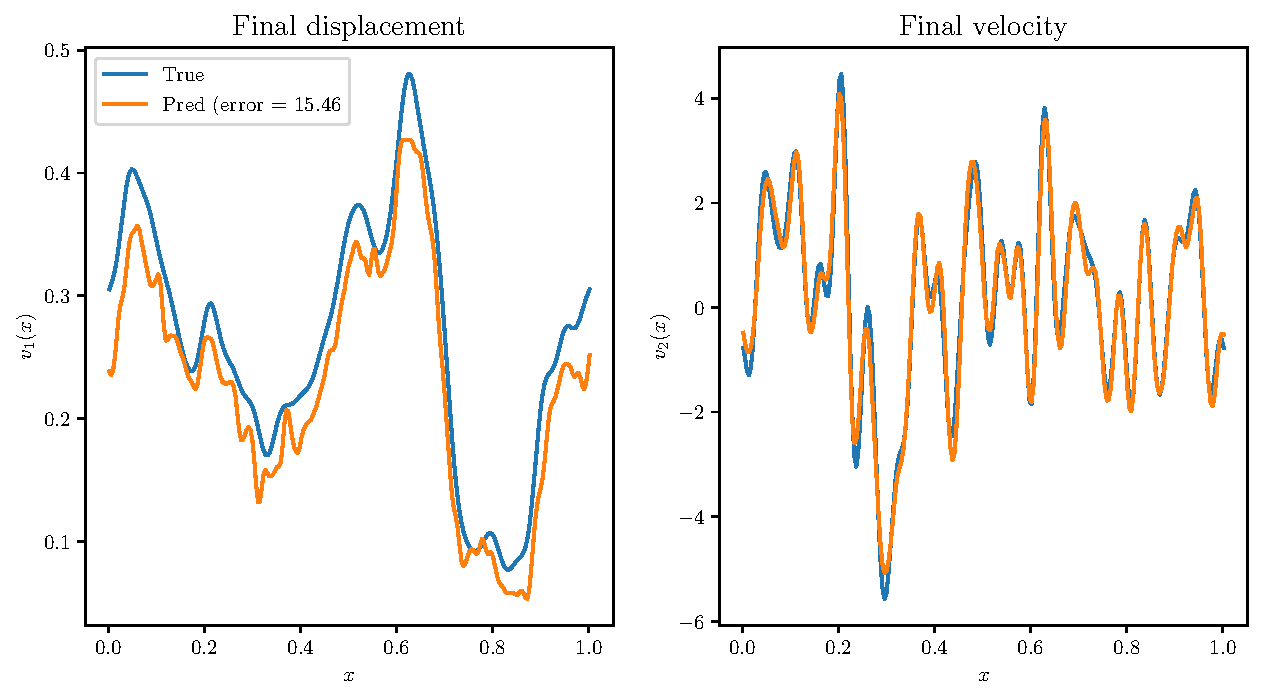
\includegraphics[width=\linewidth]{figures/wave_T=1.2.pdf}
		\caption{Example final state for the 1D wave equation (here we predict both the final displacement field and velocity field as a vector-valued target), using the same initial state as in the heat equation in Figure \ref{fig:heat_1d}---we use dimensionless units in both equations to allow direct comparison. We can see that the final states here are more oscillatory than in the heat equation in Figure \ref{fig:heat_1d}, and the operator learning model makes less accurate predictions (15.46\% relative $L^2$ error).}
		\label{fig:wave_1d}
	\end{figure}
	
	
	% ==========================================================
	% Figure 10
	% ==========================================================
	\begin{figure}[htb!]
		\centering
		\begin{subfigure}[t]{0.49\linewidth}
			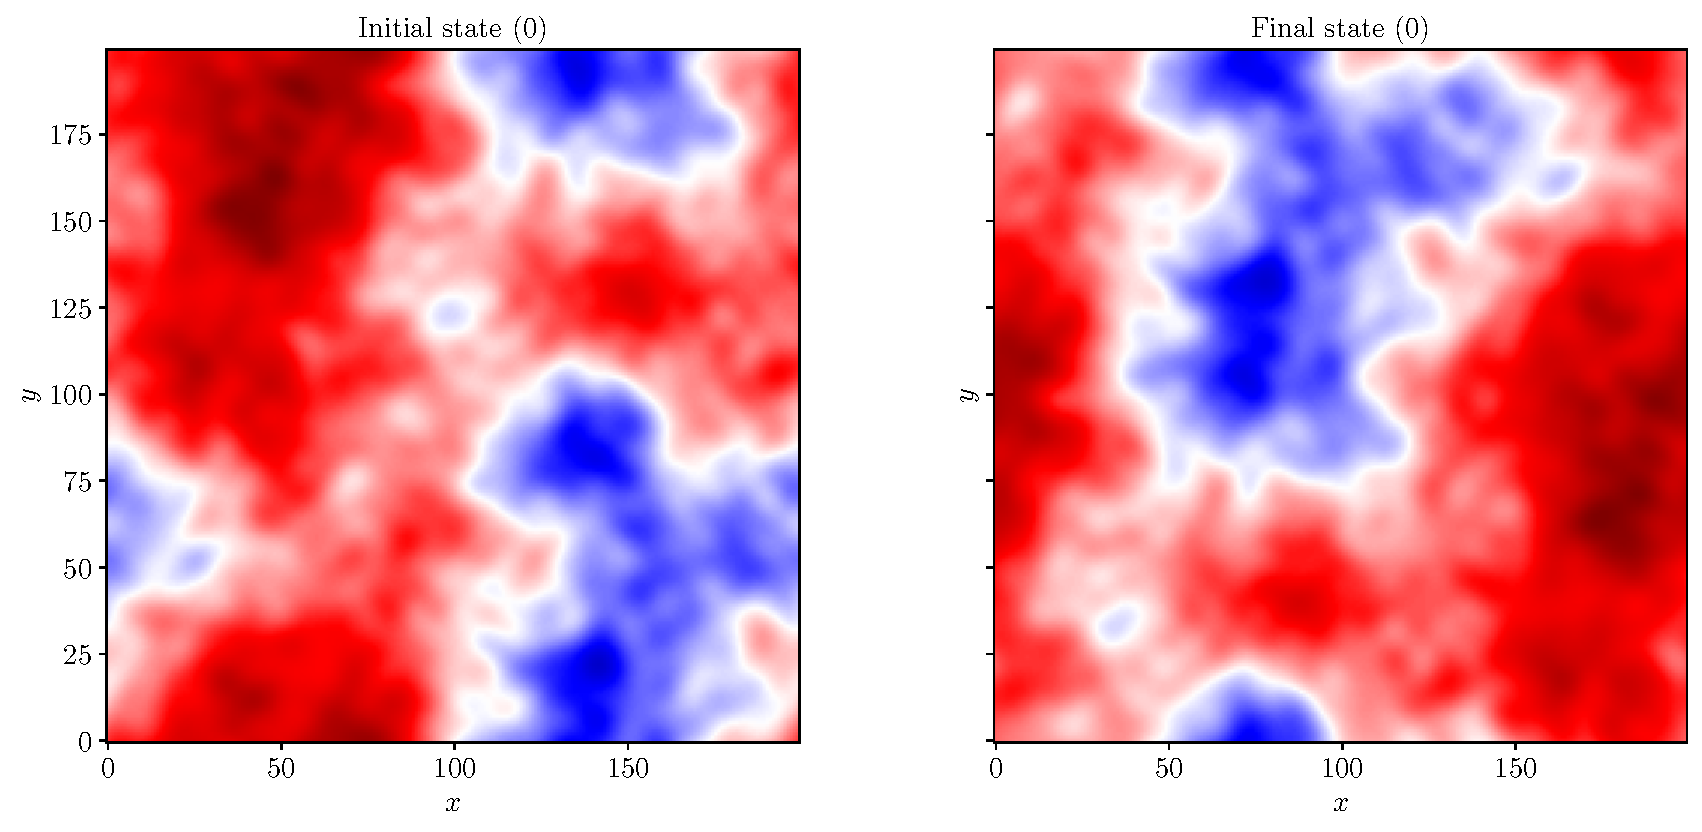
\includegraphics[width=\textwidth]{figures/ad2d-1.pdf}
			\subcaption{$k=k_0$}
		\end{subfigure}
		~
		\begin{subfigure}[t]{0.49\linewidth}
			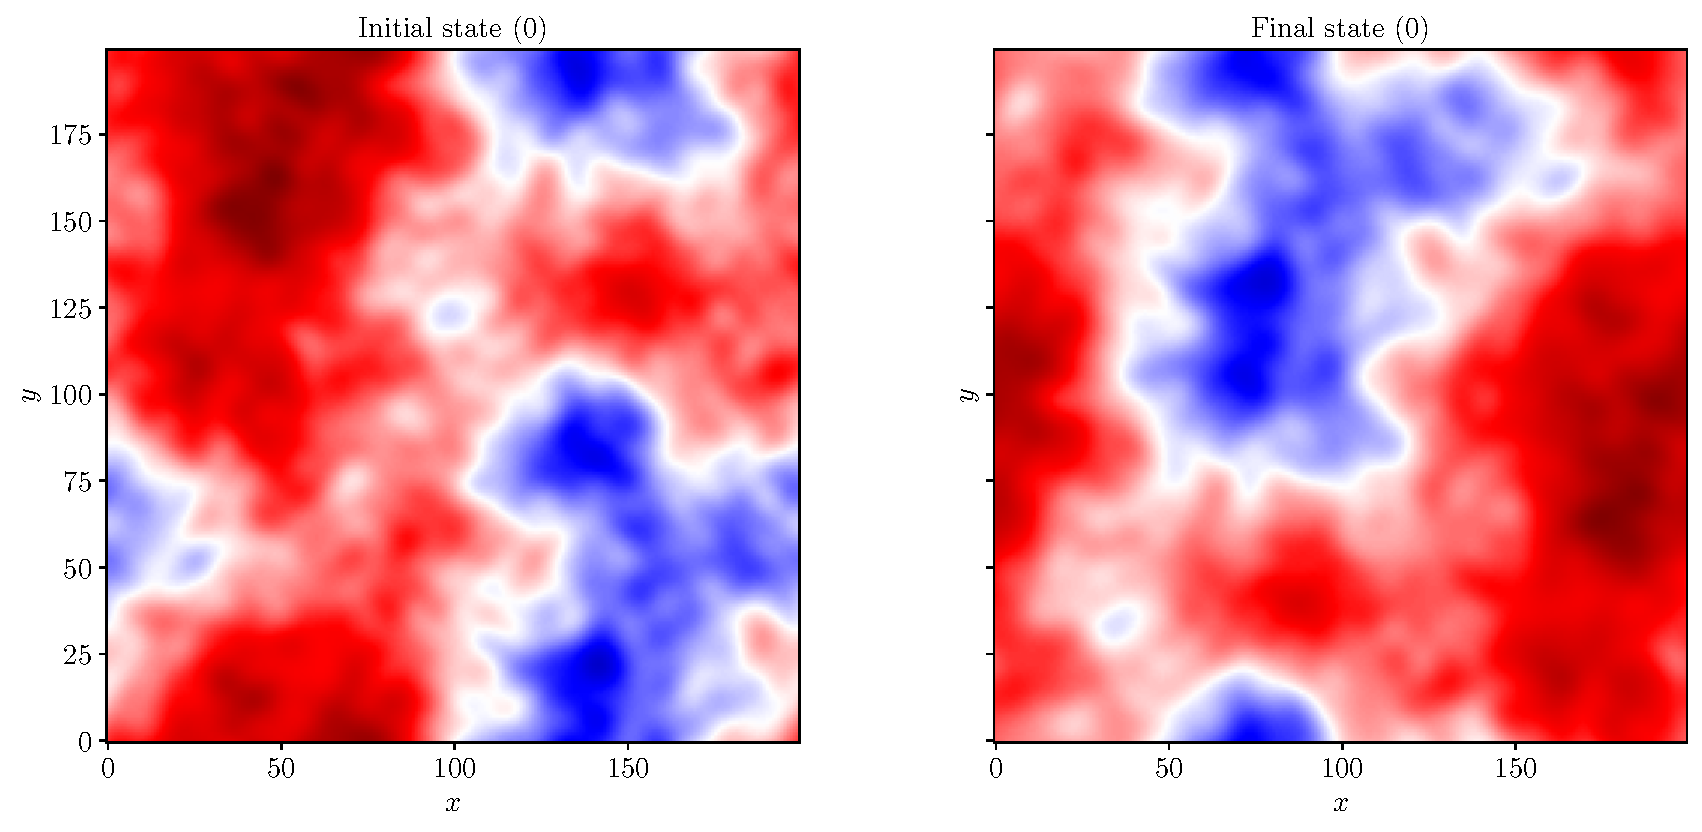
\includegraphics[width=\textwidth]{figures/ad2d-2.pdf}
			\subcaption{$k=5k_0$}
		\end{subfigure}
		~
		\begin{subfigure}[t]{0.49\linewidth}
			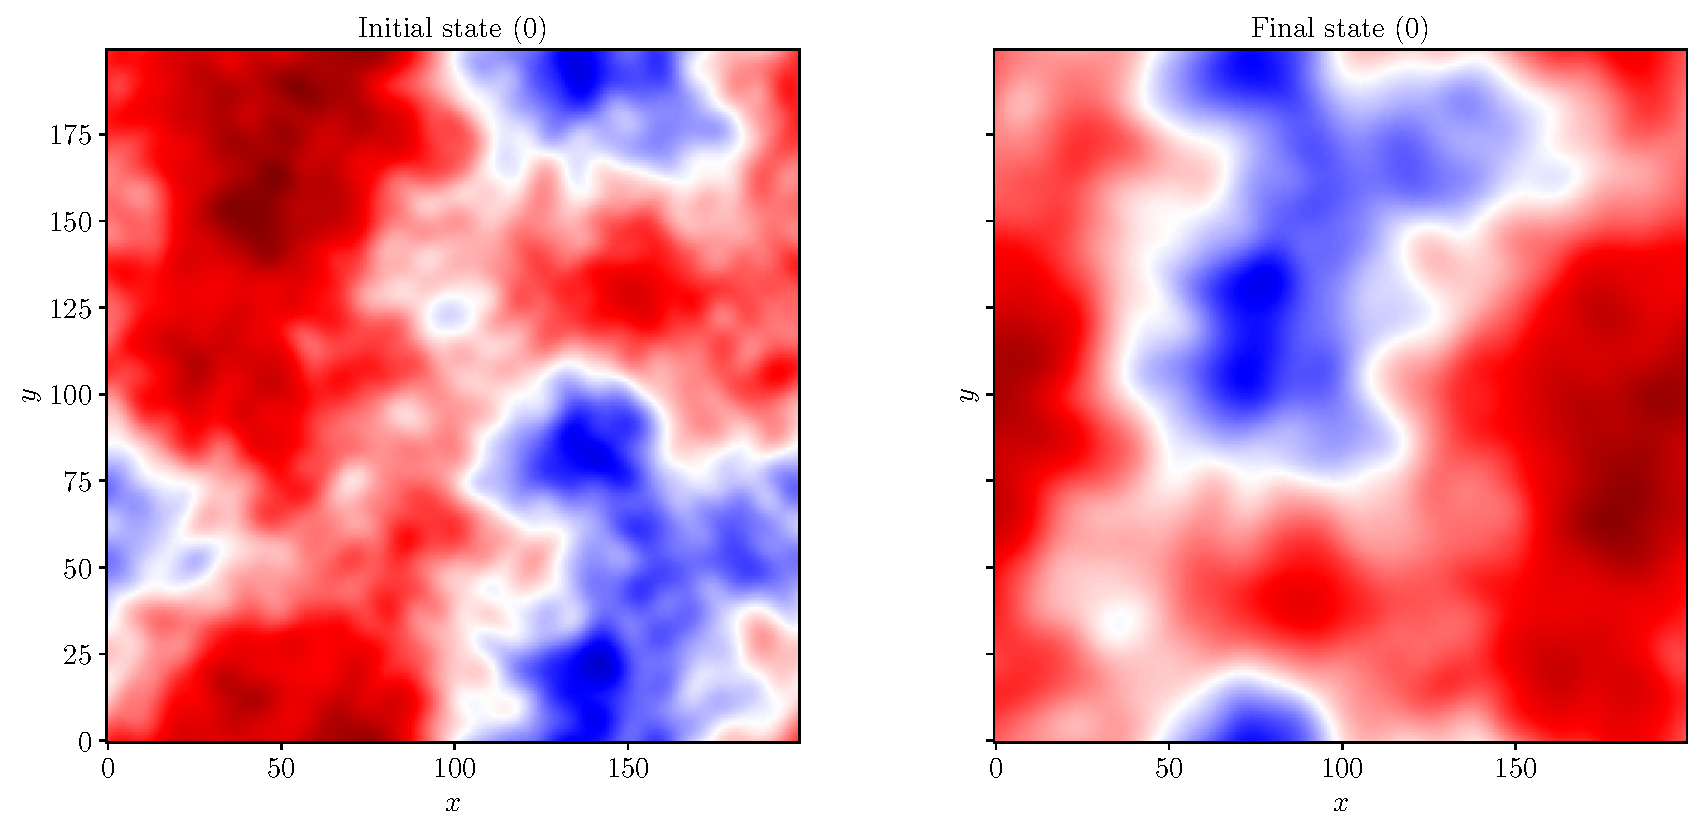
\includegraphics[width=\textwidth]{figures/ad2d-3.pdf}
			\subcaption{$k=25k_0$}
		\end{subfigure}
		~
		\begin{subfigure}[t]{0.49\linewidth}
		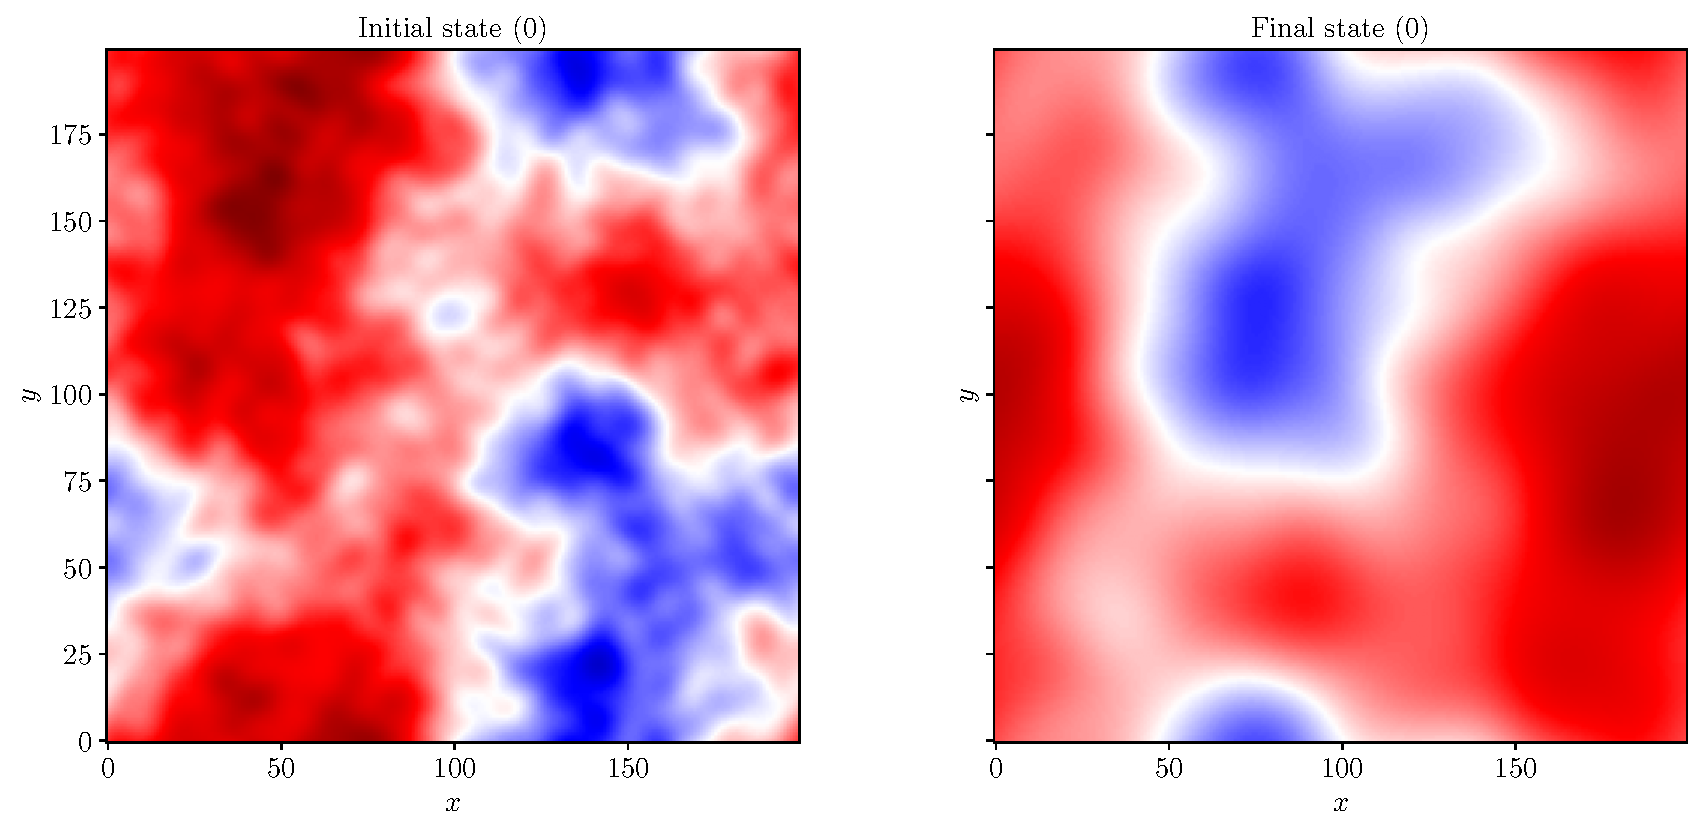
\includegraphics[width=\textwidth]{figures/ad2d-4.pdf}
		\subcaption{$k=125k_0$}
		\end{subfigure}
		\caption{Sample input and output functions for the 2D advection--diffusion equation with different values of the diffusion constant $k$. Since the same seed was used to generate each dataset, the initial state (left function in (a--d)) is the same in all cases, but the final state (right function in (a--d)) becomes smoother as $k$ increases because the physics become more diffusion-dominated. We expect to use these datasets to show that operator learning consequently has higher performance for higher values of $k$, that is, when the hyperbolic behavior of the advection term is more dominated by the parabolic behavior of the diffusion term.}
	\end{figure}
	
	% ==========================================================
	% Figure 11
	% ==========================================================
	\begin{figure}[htb!]
		\centering
		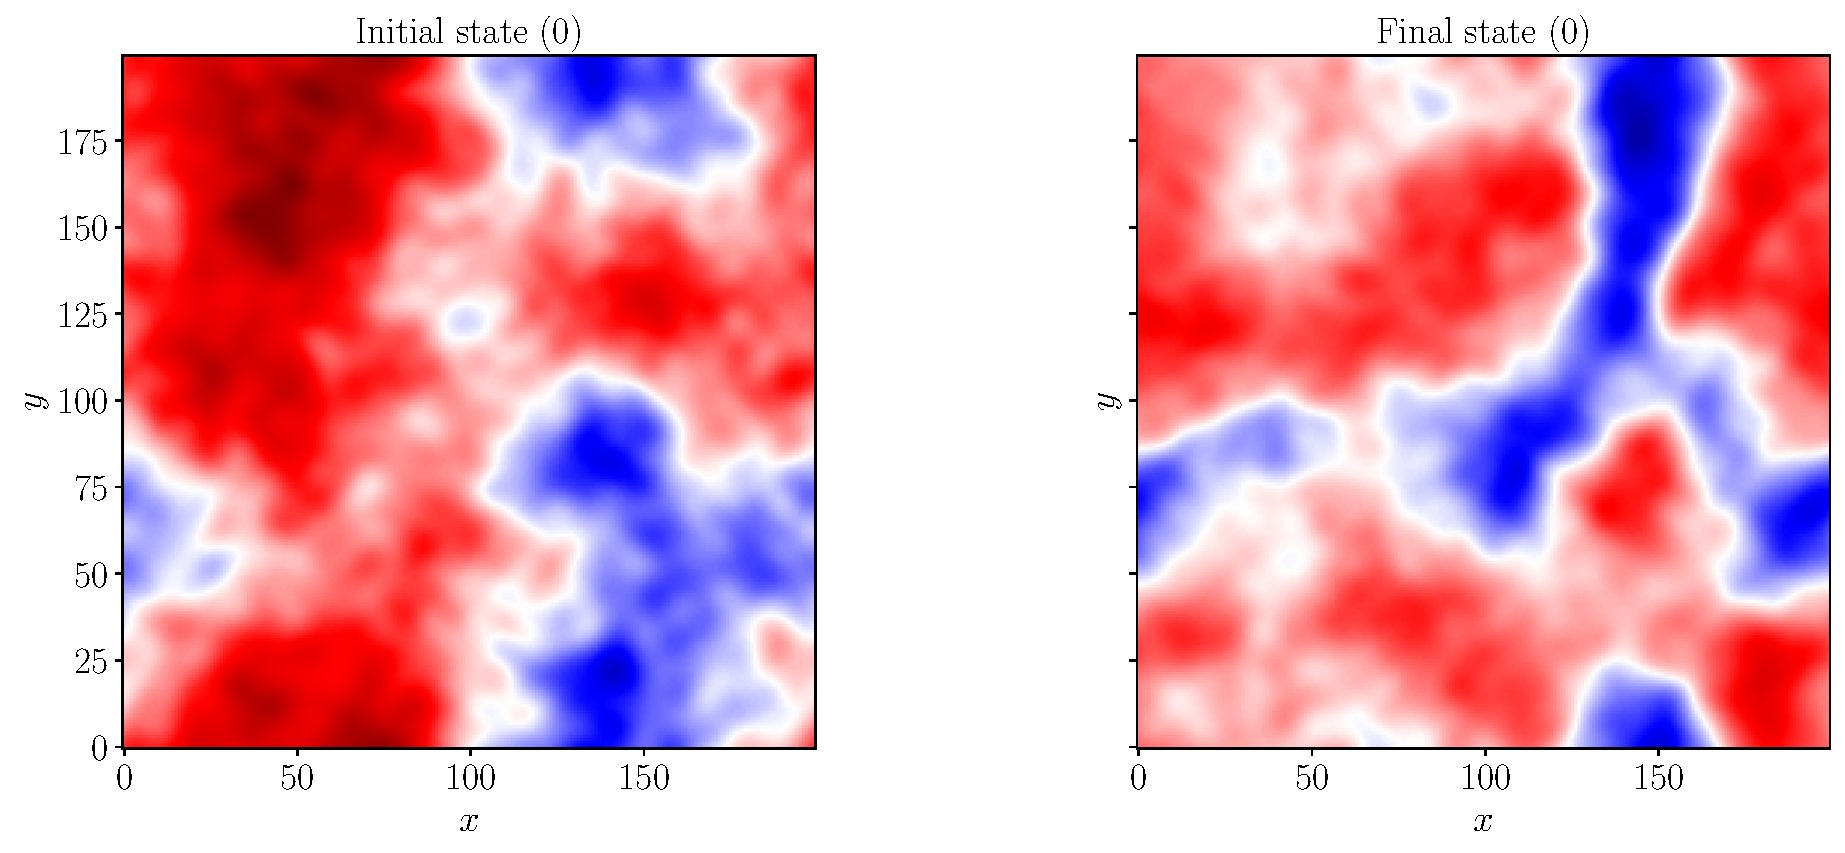
\includegraphics[width=\linewidth]{figures/nonlinear-train-0.pdf}
		\caption{Sample initial and final states from the nonlinear wave equation dataset. For planned operator learning experiments, the input is the left function and the output is the right function.}
	\end{figure}
	
	% ==========================================================
	% Figure 12
	% ==========================================================
	\begin{figure}[htb!]
		\centering
		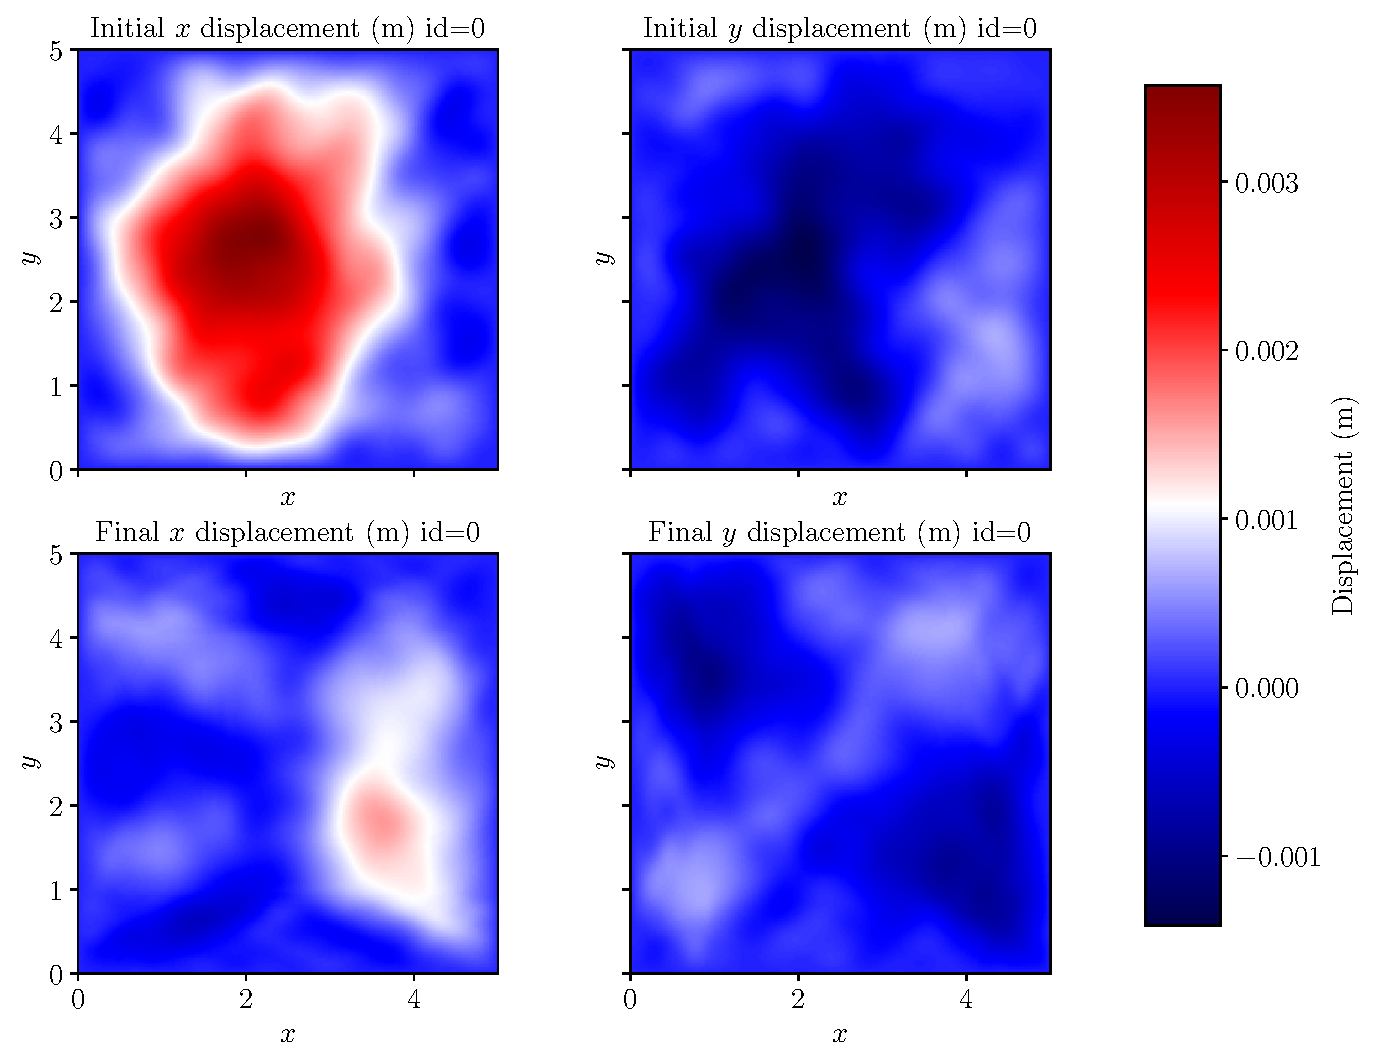
\includegraphics[width=0.9\linewidth]{figures/elasticity-0.pdf}
		\caption{Sample initial and final states from the classical elasticity dataset. For planned operator learning experiments, the input is the top row and the output is the bottom row; the left column is the $x$ displacement, and the right column is the $y$ displacement.}
	\end{figure}
	
	
	% ==========================================================
	% Figure 13
	% ==========================================================
	\begin{figure}[htb!]
		\centering
		\begin{subfigure}[t]{0.49\linewidth}
			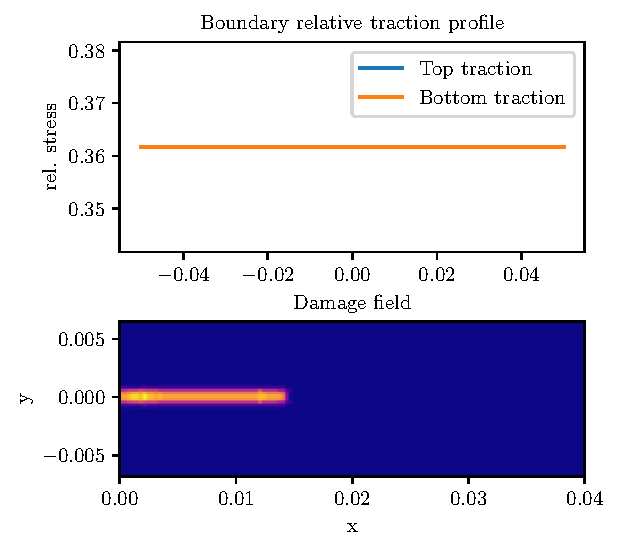
\includegraphics[width=\linewidth]{figures/sym_uniform_290.pdf}
			\subcaption{Symmetric, uniform traction}
		\end{subfigure}
		~
		\begin{subfigure}[t]{0.49\linewidth}
			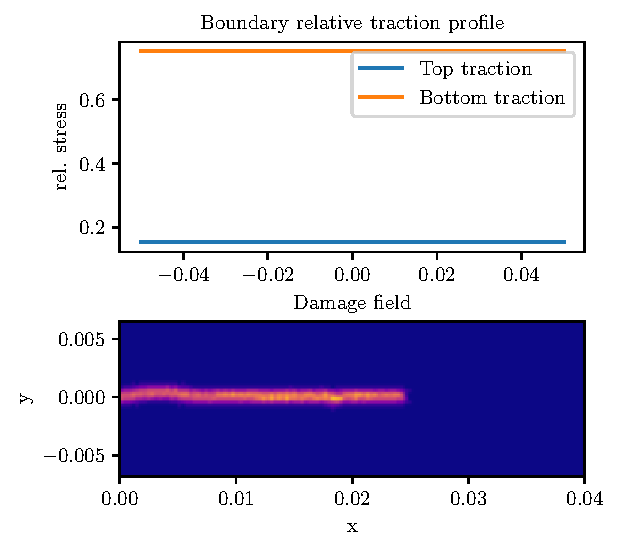
\includegraphics[width=\linewidth]{figures/asym_uniform_65.pdf}
			\subcaption{Asymmetric, uniform traction}
		\end{subfigure}
		~
		\begin{subfigure}[t]{0.49\linewidth}
			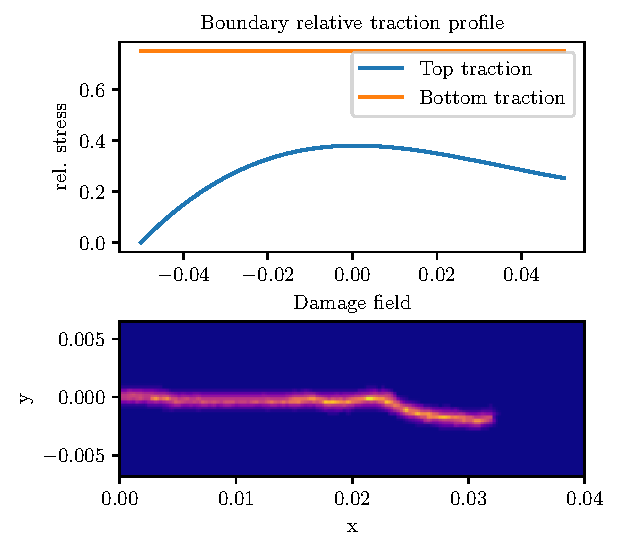
\includegraphics[width=\linewidth]{figures/asym_nonuniform_324.pdf}
			\subcaption{Asymmetric, uniform traction}
		\end{subfigure}
		\caption{Samples from generated crack propagation datasets. The input function is the boundary relative traction profile (top row, units are relative to a fixed, maximum traction), and the output function is the final damage field (bottom row, cropped to the region around where the crack grew). Note that dark blue means no damage, and orange/white means high damage. The goal for operator learning on these datasets is to predict the final crack path.}
	\end{figure}
	
	% ==========================================================
	% Figure 14
	% ==========================================================
	\begin{figure}[htb!]
		\centering
		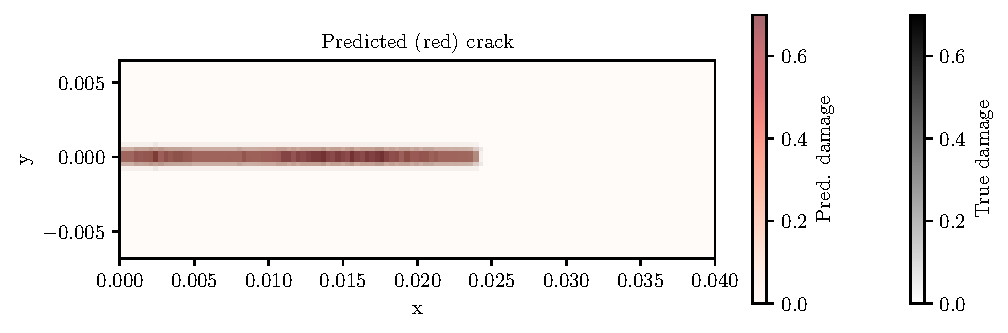
\includegraphics[width=\linewidth]{figures/compare_200.pdf}
		\caption{An example crack final damage field (black) and model prediction superimposed (red) in the case of symmetric traction on the top and bottom of the plate. This image is cropped to show only the part of the crack that grew. Note that the damage field refers to the fraction of broken bonds (between 0 and 1) per particle. The model prediction agrees closely with the true crack path.}
	\end{figure}
	
	% ==========================================================
	% Figure 15
	% ==========================================================
	\begin{figure}[htb!]
	\centering
	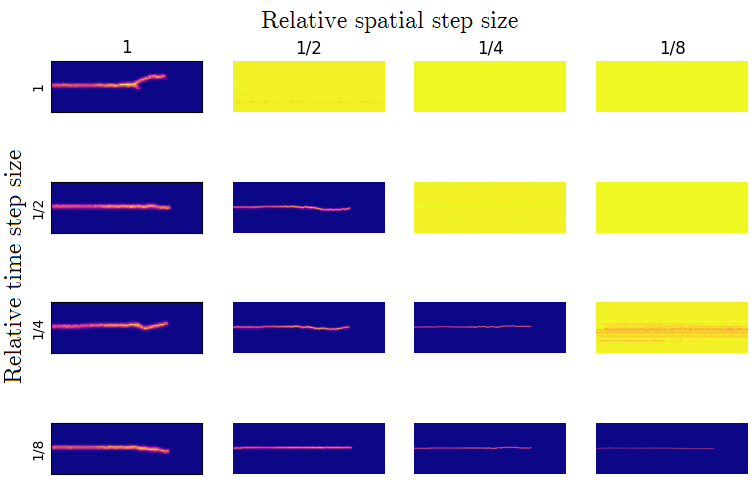
\includegraphics[width=\linewidth]{figures/comparison.png}
	\caption{Study of numerical convergence of crack propagation with asymmetric, constant loading with respect to discretization parameters. Each column corresponds to a fixed grid spacing $\Delta x$ and each row corresponds to a fixed time step size $\Delta t$ in the numerical simulation. The same peridynamic horizon $\delta$ is used in all examples. Yellow indicates numerically unstable cases (caused by the time step size being above the maximum stable time step size for the grid spacing $\Delta x$). We expect convergence to a common solution as $\Delta x$ and $\Delta t$ decrease, but the results highlight the solution’s sensitivity to the discretization parameters.}
	\end{figure}
	
	% ==========================================================
	% Figure 16
	% ==========================================================
	\begin{figure}[htb!]
		\centering
		\begin{subfigure}[t]{0.49\linewidth}
			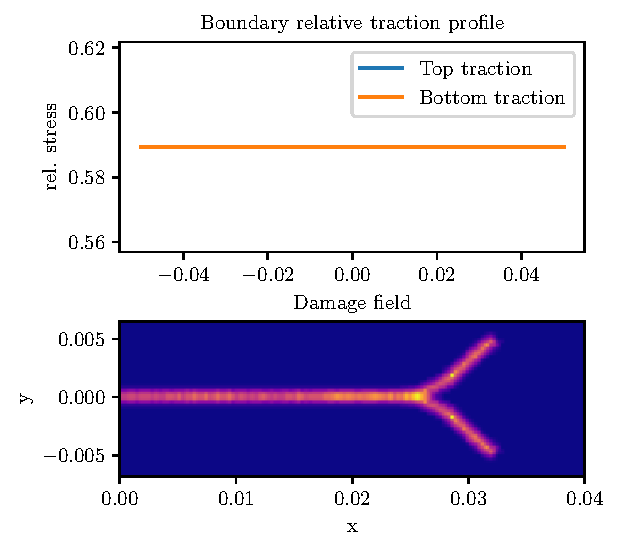
\includegraphics[width=\linewidth]{figures/unstable_118.pdf}
		\end{subfigure}
		~
		\begin{subfigure}[t]{0.49\linewidth}
			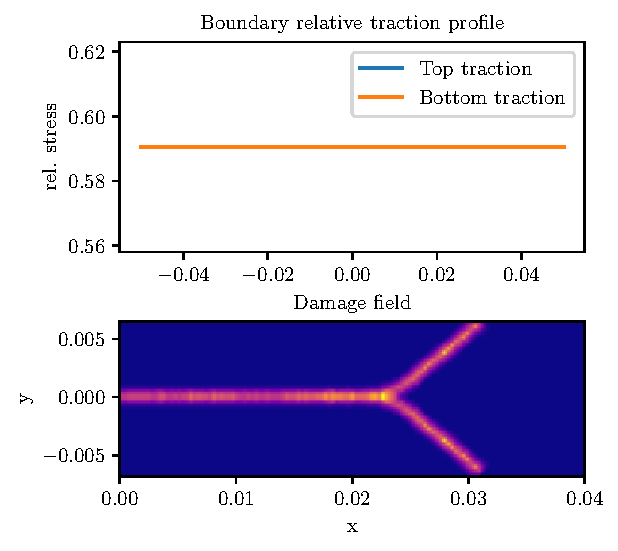
\includegraphics[width=\linewidth]{figures/unstable_119.pdf}
		\end{subfigure}
		\caption{Comparison of simulated crack paths with symmetric, uniform relative traction that differs in strength by less than 1\%, as depicted in the top two plots, which are nearly indistinguishable as a result. The simulation produces very different results despite the nearly identical parameters. This makes prediction with operator learning quite challenging, so identifying a stable configuration will be a top priority for future work following my internship.}
	\end{figure}
	
	
	% ==========================================================
	% Figure 17
	% ==========================================================
	\begin{figure}[htb!]
	\centering
	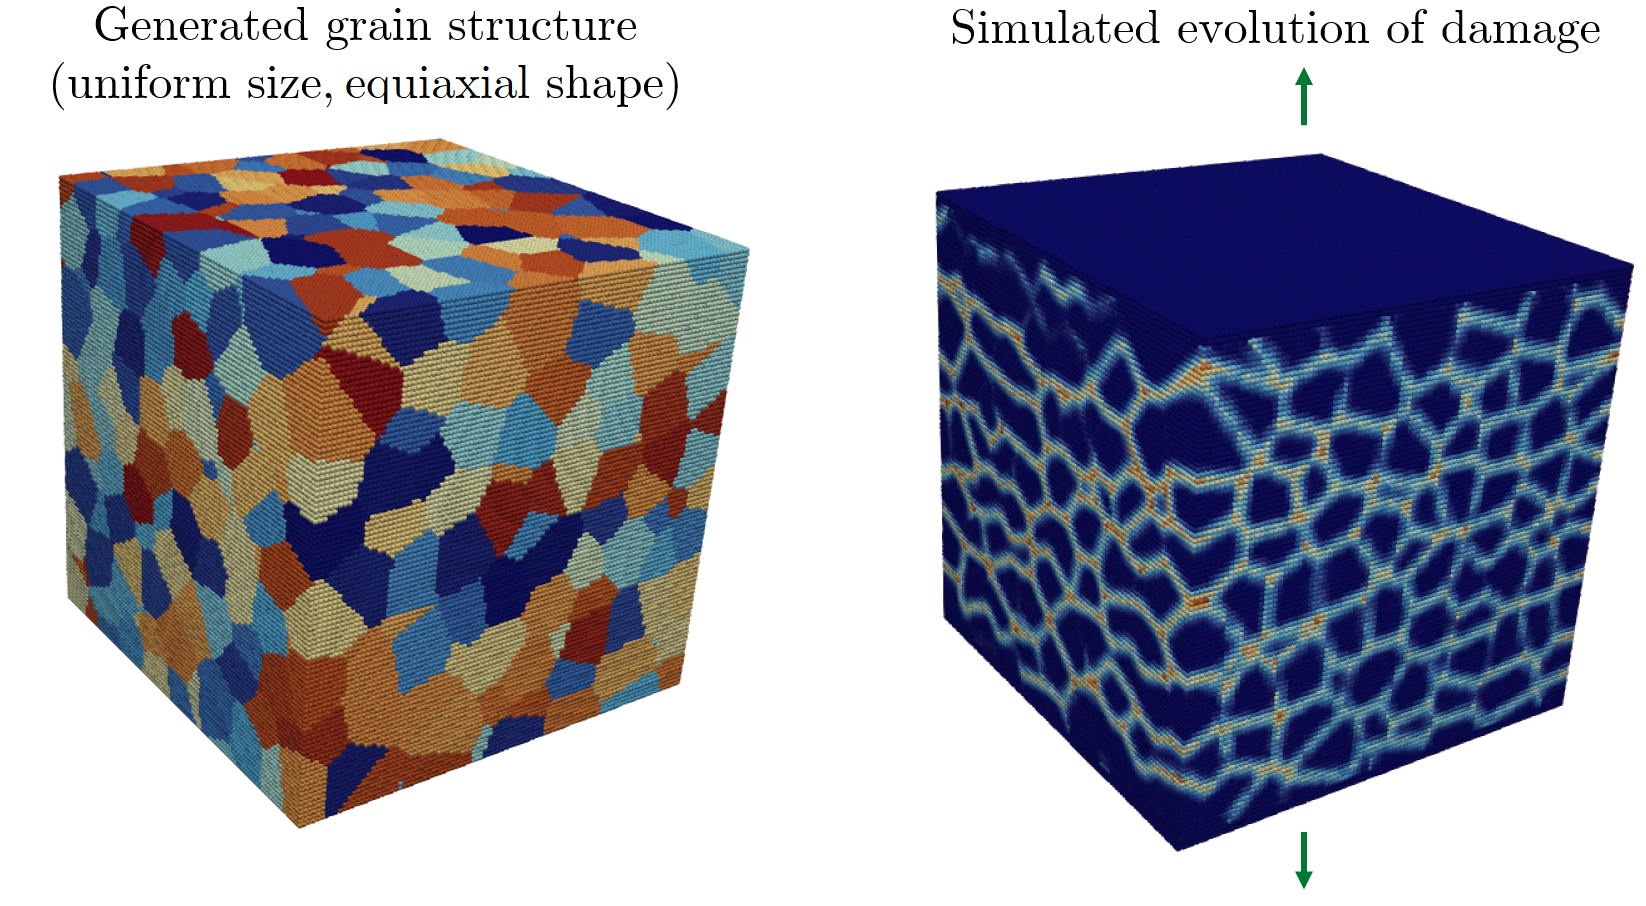
\includegraphics[width=\linewidth]{figures/voronoi_polycrystal.png}
	\caption{Left: example grain structure from my custom Voronoi tessellation algorithm that is integrated into CabanaPD. Right: final damage field (yellow, orange, and red indicate high damage, and blue indicates no damage) simulated in CabanaPD as a result of vertical tensile loading. In this demonstration, the bonds between particles in the same grain are much stronger than the bonds between particles in different grains, which is why the damage follows the grain structure. A no-fail condition is enforced on the top and bottom planes where the force is applied, so no damage is visible in these regions.}
	\end{figure}
	
	
	% ==========================================================
	% Figure 18
	% ==========================================================
	\begin{figure}[htb!]
		\centering
		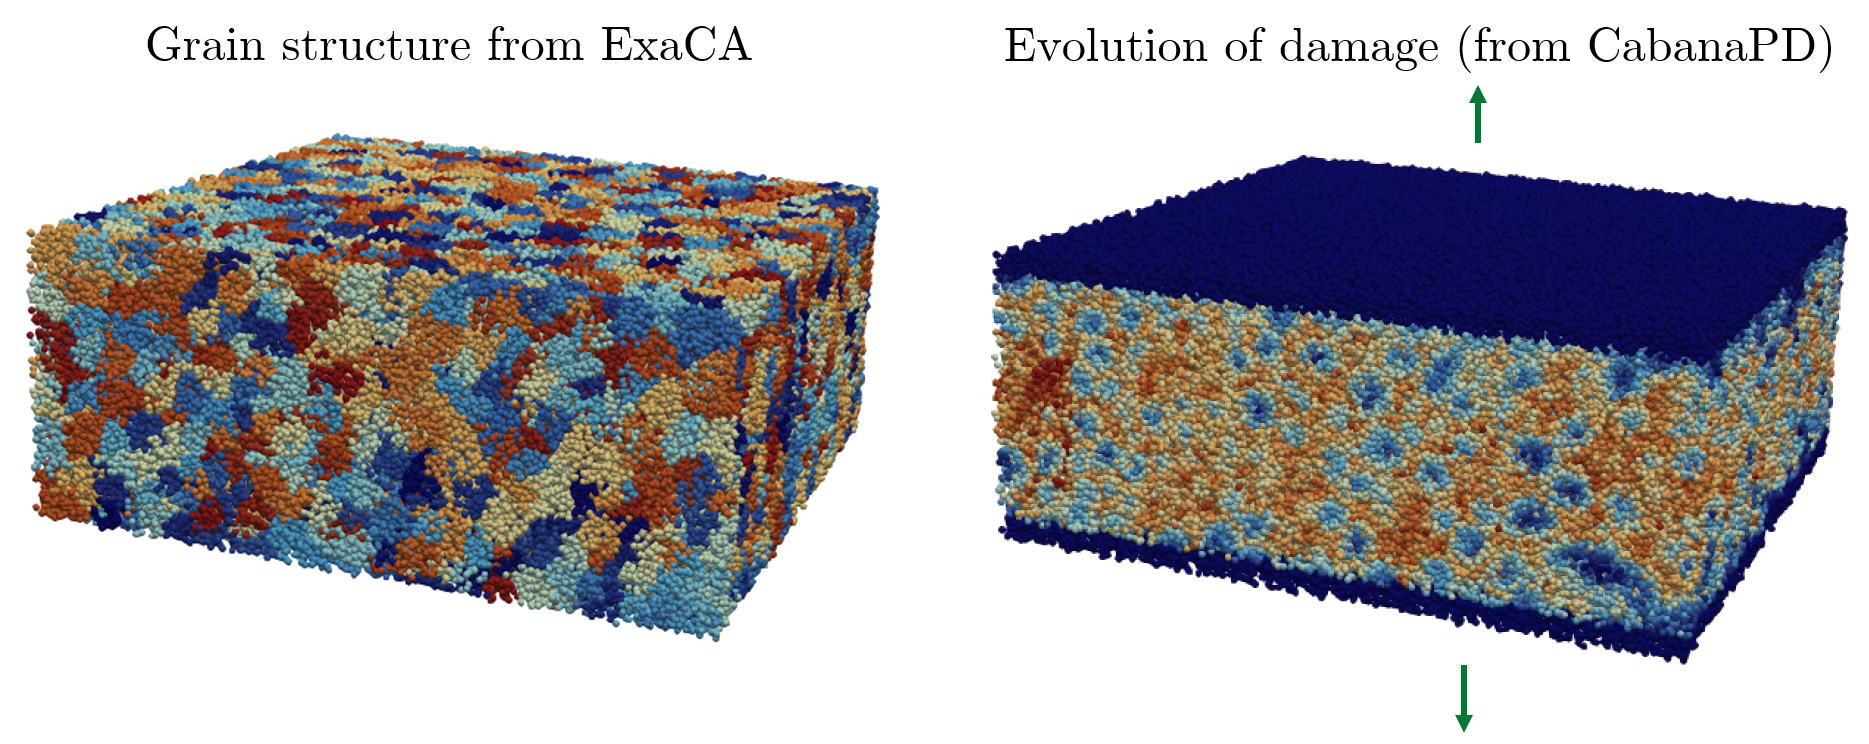
\includegraphics[width=\linewidth]{figures/exaca_polycrystal.png}
		\caption{Left: example grain structure generated using ExaCA. Right: final damage field (yellow, orange, and red indicate high damage, and blue indicates no damage) simulated in CabanaPD as a result of vertical tensile loading. In this demonstration, the bonds between particles in the same grain are much stronger than the bonds between particles in different grains, which is why the damage follows the grain structure. A no-fail condition is enforced on the top and bottom planes where the force is applied, so no damage is visible in these regions.}
	\end{figure}
	
	
\end{document}
